% Example 32: CNN Forward Pass
% A convolutional neural network processing a configurable input image.
% Feature maps are computed from the actual input pixel values via convolution.
% Change the input pixel grid below to see the network respond differently.
%
% Architecture: Input(8x8) -> Conv1(3x3, 3 filters) -> ReLU -> MaxPool(2x2)
%               -> Flatten(27) -> FC(10) -> Output
%
% Parameter: \PARAM (forward-pass progress, 0 to 1)
% Range: 0 to 1, recommended 120 frames
% Difficulty: advanced
% Features demonstrated: CNN, computed convolutions, input-responsive output
\documentclass[tikz]{standalone}
\usepackage{tikz}
\usepackage{xcolor}
\usetikzlibrary{calc, arrows.meta}

% Brand Colors
\definecolor{garnet}{HTML}{73000A}
\definecolor{rose}{HTML}{CC2E40}
\definecolor{atlantic}{HTML}{466A9F}
\definecolor{congaree}{HTML}{1F414D}
\definecolor{horseshoe}{HTML}{65780B}
\definecolor{grass}{HTML}{CED318}
\definecolor{honeycomb}{HTML}{A49137}
\definecolor{warmgrey}{HTML}{676156}
\definecolor{sandstorm}{HTML}{FFF2E3}
\definecolor{darktext}{HTML}{363636}

% Fallback so the file compiles standalone (tikzgif replaces \PARAM)
\ifdefined\PARAM\else\def\PARAM{0.65}\fi

% ================================================================
%  CONFIGURABLE INPUT IMAGE  (8x8, values 0.0-1.0, row-major)
%  Change these 64 values to any digit / pattern you like.
%  The convolution feature maps and output scores will change.
% ================================================================
%  Current pattern: digit "3"
\def\inputpixels{%
  0.0, 0.0, 0.2, 0.9, 0.9, 0.2, 0.0, 0.0,%
  0.0, 0.1, 0.8, 0.3, 0.3, 0.9, 0.1, 0.0,%
  0.0, 0.0, 0.0, 0.0, 0.1, 0.8, 0.1, 0.0,%
  0.0, 0.0, 0.1, 0.7, 0.9, 0.4, 0.0, 0.0,%
  0.0, 0.0, 0.0, 0.0, 0.1, 0.8, 0.1, 0.0,%
  0.0, 0.0, 0.0, 0.0, 0.1, 0.8, 0.1, 0.0,%
  0.0, 0.1, 0.8, 0.3, 0.3, 0.9, 0.1, 0.0,%
  0.0, 0.0, 0.2, 0.9, 0.9, 0.2, 0.0, 0.0%
}

% ================================================================
%  CONVOLUTION HELPERS
%  Three 3x3 filters: horizontal-edge, vertical-edge, center-surround
% ================================================================
%  doconvH : kernel = [-1 -1 -1; 0 0 0; 1 1 1]  (horizontal edges)
\newcommand{\doconvH}[2]{%
  \pgfmathsetmacro{\convresult}{max(0,%
    -array({\inputpixels},(#1)*8+(#2))%
    -array({\inputpixels},(#1)*8+(#2)+1)%
    -array({\inputpixels},(#1)*8+(#2)+2)%
    +array({\inputpixels},(#1+2)*8+(#2))%
    +array({\inputpixels},(#1+2)*8+(#2)+1)%
    +array({\inputpixels},(#1+2)*8+(#2)+2)%
  )}%
}
%  doconvV : kernel = [-1 0 1; -1 0 1; -1 0 1]  (vertical edges)
\newcommand{\doconvV}[2]{%
  \pgfmathsetmacro{\convresult}{max(0,%
    -array({\inputpixels},(#1)*8+(#2))%
    +array({\inputpixels},(#1)*8+(#2)+2)%
    -array({\inputpixels},(#1+1)*8+(#2))%
    +array({\inputpixels},(#1+1)*8+(#2)+2)%
    -array({\inputpixels},(#1+2)*8+(#2))%
    +array({\inputpixels},(#1+2)*8+(#2)+2)%
  )}%
}
%  doconvC : kernel = [-1 -1 -1; -1 8 -1; -1 -1 -1]  (blob / center-surround)
\newcommand{\doconvC}[2]{%
  \pgfmathsetmacro{\convresult}{max(0,%
    -array({\inputpixels},(#1)*8+(#2))%
    -array({\inputpixels},(#1)*8+(#2)+1)%
    -array({\inputpixels},(#1)*8+(#2)+2)%
    -array({\inputpixels},(#1+1)*8+(#2))%
    +8*array({\inputpixels},(#1+1)*8+(#2)+1)%
    -array({\inputpixels},(#1+1)*8+(#2)+2)%
    -array({\inputpixels},(#1+2)*8+(#2))%
    -array({\inputpixels},(#1+2)*8+(#2)+1)%
    -array({\inputpixels},(#1+2)*8+(#2)+2)%
  )}%
}

\begin{document}
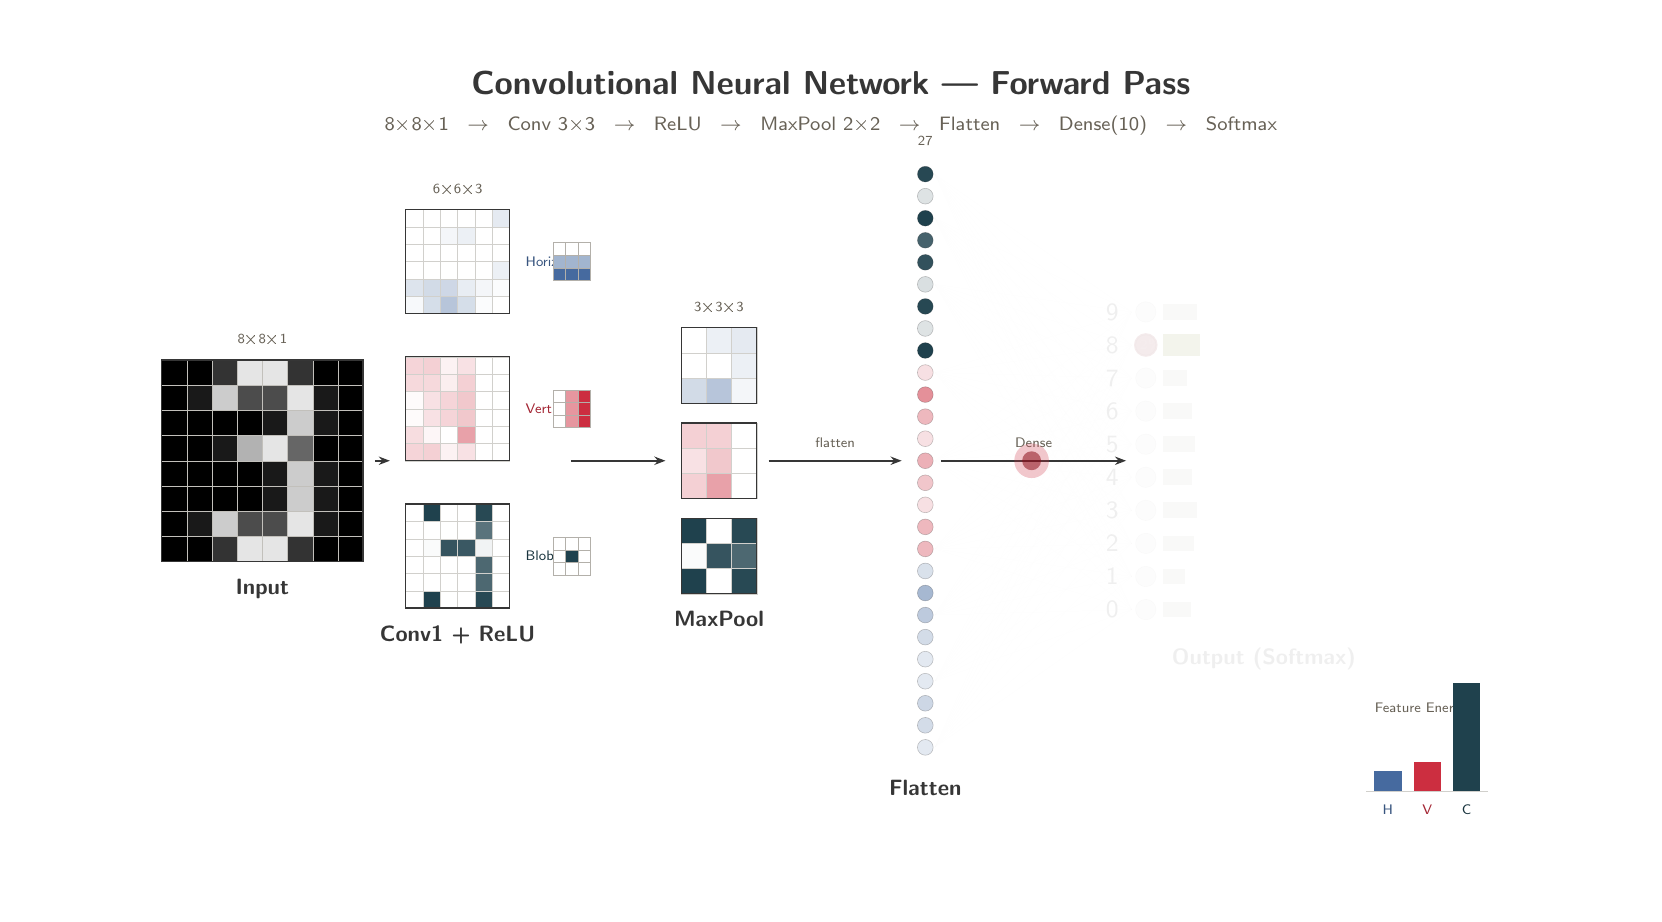
\begin{tikzpicture}
  \useasboundingbox (-10.2,-5.5) rectangle (10.2,5.5);

  % Animation parameter (0 to 1)
  \pgfmathsetmacro{\t}{\PARAM}

  % === PHASE THRESHOLDS ===
  \pgfmathsetmacro{\tConv}{0.18}     % conv starts filling
  \pgfmathsetmacro{\tConvEnd}{0.38}  % conv done
  \pgfmathsetmacro{\tPool}{0.45}     % pool visible
  \pgfmathsetmacro{\tFC}{0.62}       % FC visible
  \pgfmathsetmacro{\tOut}{0.80}      % output visible

  % Layer opacities (fade in over 0.08 of progress)
  \pgfmathsetmacro{\opConv}{min(1, max(0.08, (\t-\tConv+0.08)/0.08))}
  \pgfmathsetmacro{\opPool}{min(1, max(0.08, (\t-\tPool+0.08)/0.08))}
  \pgfmathsetmacro{\opFC}{min(1, max(0.08, (\t-\tFC+0.08)/0.08))}
  \pgfmathsetmacro{\opOut}{min(1, max(0.08, (\t-\tOut+0.08)/0.08))}

  % ============================================================
  %  PRE-COMPUTE ALL CONV1 VALUES  (3 filters x 6x6 = 108 values)
  % ============================================================
  % Store globally so they survive foreach scoping.
  % Naming: \cvH0 .. \cvH35,  \cvV0 .. \cvV35,  \cvC0 .. \cvC35

  % --- Filter H (horizontal edges) ---
  \foreach \ci in {0,...,5}{%
    \foreach \cj in {0,...,5}{%
      \doconvH{\ci}{\cj}%
      \pgfmathtruncatemacro{\idx}{\ci*6+\cj}%
      \expandafter\xdef\csname cvH\idx\endcsname{\convresult}%
    }%
  }
  % --- Filter V (vertical edges) ---
  \foreach \ci in {0,...,5}{%
    \foreach \cj in {0,...,5}{%
      \doconvV{\ci}{\cj}%
      \pgfmathtruncatemacro{\idx}{\ci*6+\cj}%
      \expandafter\xdef\csname cvV\idx\endcsname{\convresult}%
    }%
  }
  % --- Filter C (center-surround) ---
  \foreach \ci in {0,...,5}{%
    \foreach \cj in {0,...,5}{%
      \doconvC{\ci}{\cj}%
      \pgfmathtruncatemacro{\idx}{\ci*6+\cj}%
      \expandafter\xdef\csname cvC\idx\endcsname{\convresult}%
    }%
  }

  % Find global max for colour normalisation
  \xdef\maxcv{0.01}
  \foreach \idx in {0,...,35}{%
    \pgfmathsetmacro{\tmp}{max(max(\csname cvH\idx\endcsname,\csname cvV\idx\endcsname),\csname cvC\idx\endcsname)}%
    \pgfmathsetmacro{\newmax}{max(\maxcv,\tmp)}%
    \xdef\maxcv{\newmax}%
  }

  % ============================================================
  %  PRE-COMPUTE POOL1  (2x2 max-pool -> 3x3 per filter = 27 values)
  % ============================================================
  \foreach \f in {H,V,C}{%
    \foreach \pi in {0,1,2}{%
      \foreach \pj in {0,1,2}{%
        \pgfmathtruncatemacro{\idA}{(2*\pi)*6  +(2*\pj)}%
        \pgfmathtruncatemacro{\idB}{(2*\pi)*6  +(2*\pj+1)}%
        \pgfmathtruncatemacro{\idC}{(2*\pi+1)*6+(2*\pj)}%
        \pgfmathtruncatemacro{\idD}{(2*\pi+1)*6+(2*\pj+1)}%
        \pgfmathsetmacro{\pval}{max(%
          max(\csname cv\f\idA\endcsname,\csname cv\f\idB\endcsname),%
          max(\csname cv\f\idC\endcsname,\csname cv\f\idD\endcsname)%
        )}%
        \pgfmathtruncatemacro{\pidx}{\pi*3+\pj}%
        \expandafter\xdef\csname pl\f\pidx\endcsname{\pval}%
      }%
    }%
  }

  % Pool max for normalisation
  \xdef\maxpl{0.01}
  \foreach \f in {H,V,C}{%
    \foreach \pidx in {0,...,8}{%
      \pgfmathsetmacro{\newmax}{max(\maxpl,\csname pl\f\pidx\endcsname)}%
      \xdef\maxpl{\newmax}%
    }%
  }

  % ============================================================
  %  COMPUTE FEATURE ENERGIES  -> OUTPUT SCORES
  % ============================================================
  \xdef\eH{0}\xdef\eV{0}\xdef\eC{0}
  \foreach \pidx in {0,...,8}{%
    \pgfmathsetmacro{\newH}{\eH+\csname plH\pidx\endcsname}%
    \pgfmathsetmacro{\newV}{\eV+\csname plV\pidx\endcsname}%
    \pgfmathsetmacro{\newC}{\eC+\csname plC\pidx\endcsname}%
    \xdef\eH{\newH}\xdef\eV{\newV}\xdef\eC{\newC}%
  }
  \pgfmathsetmacro{\eTotal}{max(0.01, \eH+\eV+\eC)}
  \pgfmathsetmacro{\fH}{\eH/\eTotal}
  \pgfmathsetmacro{\fV}{\eV/\eTotal}
  \pgfmathsetmacro{\fC}{\eC/\eTotal}

  % 10 output scores from a simple pseudo-weight matrix
  % Each class favours a different feature mix
  \pgfmathsetmacro{\sZero} {0.35*\fH + 0.35*\fV + 0.30*\fC + 0.01}
  \pgfmathsetmacro{\sOne}  {0.05*\fH + 0.85*\fV + 0.10*\fC + 0.02}
  \pgfmathsetmacro{\sTwo}  {0.45*\fH + 0.15*\fV + 0.40*\fC + 0.00}
  \pgfmathsetmacro{\sThree}{0.50*\fH + 0.10*\fV + 0.40*\fC + 0.03}
  \pgfmathsetmacro{\sFour} {0.15*\fH + 0.55*\fV + 0.30*\fC + 0.00}
  \pgfmathsetmacro{\sFive} {0.55*\fH + 0.05*\fV + 0.40*\fC + 0.01}
  \pgfmathsetmacro{\sSix}  {0.40*\fH + 0.25*\fV + 0.35*\fC + 0.00}
  \pgfmathsetmacro{\sSeven}{0.30*\fH + 0.50*\fV + 0.20*\fC + 0.01}
  \pgfmathsetmacro{\sEight}{0.25*\fH + 0.25*\fV + 0.50*\fC + 0.00}
  \pgfmathsetmacro{\sNine} {0.20*\fH + 0.40*\fV + 0.40*\fC + 0.01}

  % Normalise scores to probabilities (simple sum-normalisation)
  \pgfmathsetmacro{\sSum}{\sZero+\sOne+\sTwo+\sThree+\sFour+\sFive+\sSix+\sSeven+\sEight+\sNine}

  % Find winner index
  \xdef\winIdx{0}\xdef\winVal{\sZero}
  \foreach \idx/\sv in {1/\sOne,2/\sTwo,3/\sThree,4/\sFour,5/\sFive,6/\sSix,7/\sSeven,8/\sEight,9/\sNine}{%
    \pgfmathsetmacro{\better}{(\sv > \winVal) ? 1 : 0}%
    \ifnum\better=1 \xdef\winIdx{\idx}\xdef\winVal{\sv}\fi%
  }

  % ============================================================
  %  DRAWING
  % ============================================================

  % --- Title ---
  \node[darktext, font=\sffamily\bfseries\large] at (0, 4.8)
    {Convolutional Neural Network --- Forward Pass};

  % --- Architecture summary ---
  \node[warmgrey, font=\sffamily\scriptsize] at (0, 4.25)
    {8\texttimes8\texttimes1 \;\;$\rightarrow$\;\;
     Conv 3\texttimes3 \;\;$\rightarrow$\;\;
     ReLU \;\;$\rightarrow$\;\;
     MaxPool 2\texttimes2 \;\;$\rightarrow$\;\;
     Flatten \;\;$\rightarrow$\;\;
     Dense(10) \;\;$\rightarrow$\;\;
     Softmax};

  % ==========  INPUT IMAGE  (8x8)  ==========
  \def\inX{-8.5}    % left edge
  \def\inY{0}       % vertical centre
  \def\cs{0.32}     % cell size
  \pgfmathsetmacro{\inW}{\cs*8}
  \begin{scope}[shift={(\inX,{\inY-\inW/2})}]
    \foreach \r in {0,...,7}{%
      \foreach \c in {0,...,7}{%
        \pgfmathtruncatemacro{\pidx}{\r*8+\c}%
        \pgfmathsetmacro{\pv}{array({\inputpixels},\pidx)}%
        \pgfmathsetmacro{\grey}{100-\pv*100}%  0→white, 1→black
        \fill[black!\grey!white] ({\c*\cs},{(7-\r)*\cs}) rectangle ({(\c+1)*\cs},{(8-\r)*\cs});
        \draw[warmgrey!40, line width=0.15pt] ({\c*\cs},{(7-\r)*\cs}) rectangle ({(\c+1)*\cs},{(8-\r)*\cs});
      }%
    }
    % Border
    \draw[darktext, line width=0.6pt] (0,0) rectangle ({\inW},{\inW});
  \end{scope}
  \node[darktext, font=\sffamily\footnotesize\bfseries, below]
    at ({\inX+\inW/2},{\inY-\inW/2-0.1}) {Input};
  \node[warmgrey, font=\sffamily\tiny, above]
    at ({\inX+\inW/2},{\inY+\inW/2+0.05}) {8\texttimes8\texttimes1};

  % --- Sliding kernel highlight on input (during conv phase) ---
  \pgfmathsetmacro{\convProgress}{min(1, max(0, (\t-0.02)/(\tConvEnd-0.02)))}
  \pgfmathtruncatemacro{\kernelPos}{min(35, floor(\convProgress*36))}
  \pgfmathtruncatemacro{\kRow}{floor(\kernelPos/6)}
  \pgfmathtruncatemacro{\kCol}{\kernelPos - \kRow*6}
  \pgfmathsetmacro{\showKernel}{(\t > 0.02 && \t < \tConvEnd) ? 1 : 0}
  \ifnum\showKernel=1
    \draw[garnet, line width=1.2pt]
      ({\inX+\kCol*\cs},{\inY+\inW/2-((\kRow)*\cs)})
      rectangle
      ({\inX+(\kCol+3)*\cs},{\inY+\inW/2-((\kRow+3)*\cs)});
  \fi

  % ==========  FLOW ARROW: Input -> Conv  ==========
  \pgfmathsetmacro{\arConv}{min(1, max(0, \t/\tConv))}
  \draw[-{Stealth[length=4pt]}, darktext, opacity=\arConv, line width=0.7pt]
    ({\inX+\inW+0.15}, \inY) -- (-5.6, \inY);

  % ==========  CONV1 FEATURE MAPS  (3 filters, 6x6 each)  ==========
  % Drawn as three grids stacked vertically
  \def\fmX{-5.4}     % left edge of feature maps
  \def\fmCS{0.22}    % cell size
  \pgfmathsetmacro{\fmW}{\fmCS*6}
  \def\fmGap{0.55}   % vertical gap between maps

  % Vertical positions for three maps
  \pgfmathsetmacro{\fmYtop}{\fmGap + \fmW}    % top of filter H map
  \pgfmathsetmacro{\fmYmid}{0}                 % centre of filter V map
  \pgfmathsetmacro{\fmYbot}{-\fmGap - \fmW}    % bottom of filter C map

  % Filter colours
  \colorlet{colH}{atlantic}
  \colorlet{colV}{rose}
  \colorlet{colC}{congaree}

  \foreach \f/\fYbase/\fcol/\flabel in {%
    H/\fmYtop/colH/Horiz,%
    V/\fmYmid/colV/Vert,%
    C/\fmYbot/colC/Blob%
  }{%
    \begin{scope}[shift={(\fmX,\fYbase)}]
      \foreach \ci in {0,...,5}{%
        \foreach \cj in {0,...,5}{%
          \pgfmathtruncatemacro{\idx}{\ci*6+\cj}%
          \pgfmathsetmacro{\val}{\csname cv\f\idx\endcsname}%
          \pgfmathsetmacro{\pct}{min(100, \val/\maxcv*100)}%
          % Only show cells the kernel has already passed (animation)
          \pgfmathsetmacro{\cellVisible}{(\idx < \kernelPos || \t >= \tConvEnd) ? 1 : 0}%
          \pgfmathsetmacro{\cellOp}{\opConv * ((\cellVisible > 0.5) ? 1.0 : 0.06)}%
          \fill[\fcol!\pct!white, opacity=\cellOp]
            ({\cj*\fmCS},{(5-\ci)*\fmCS}) rectangle ({(\cj+1)*\fmCS},{(6-\ci)*\fmCS});
          \draw[warmgrey!30, line width=0.1pt, opacity=\cellOp]
            ({\cj*\fmCS},{(5-\ci)*\fmCS}) rectangle ({(\cj+1)*\fmCS},{(6-\ci)*\fmCS});
        }%
      }%
      \draw[darktext, line width=0.4pt, opacity=\opConv] (0,0) rectangle ({\fmW},{\fmW});
      % Label
      \node[\fcol!80!black, font=\sffamily\tiny, opacity=\opConv, right]
        at ({\fmW+0.08},{\fmW/2}) {\flabel};
    \end{scope}
  }
  \node[darktext, font=\sffamily\footnotesize\bfseries, opacity=\opConv, below]
    at ({\fmX+\fmW/2},{\fmYbot-0.1}) {Conv1 + ReLU};
  \node[warmgrey, font=\sffamily\tiny, opacity=\opConv, above]
    at ({\fmX+\fmW/2},{\fmYtop+\fmW+0.05}) {6\texttimes6\texttimes3};

  % --- Kernel weight insets (small 3x3 grids beside each map) ---
  \pgfmathsetmacro{\showKernInset}{(\t > \tConv) ? 1 : 0}
  \ifnum\showKernInset=1
    % Kernel H: -1 -1 -1 / 0 0 0 / 1 1 1
    \def\kiCS{0.16}
    \begin{scope}[shift={({\fmX+\fmW+0.55},{\fmYtop+\fmW/2-1.5*\kiCS})}]
      \foreach \kr/\kc/\kv in {0/0/-1,0/1/-1,0/2/-1,1/0/0,1/1/0,1/2/0,2/0/1,2/1/1,2/2/1}{%
        \pgfmathsetmacro{\kpct}{(\kv+1)*50}%  -1->0, 0->50, 1->100
        \fill[colH!\kpct!white] ({\kc*\kiCS},{(2-\kr)*\kiCS}) rectangle ({(\kc+1)*\kiCS},{(3-\kr)*\kiCS});
        \draw[warmgrey!50, line width=0.15pt] ({\kc*\kiCS},{(2-\kr)*\kiCS}) rectangle ({(\kc+1)*\kiCS},{(3-\kr)*\kiCS});
      }
    \end{scope}
    % Kernel V
    \begin{scope}[shift={({\fmX+\fmW+0.55},{\fmYmid+\fmW/2-1.5*\kiCS})}]
      \foreach \kr/\kc/\kv in {0/0/-1,0/1/0,0/2/1,1/0/-1,1/1/0,1/2/1,2/0/-1,2/1/0,2/2/1}{%
        \pgfmathsetmacro{\kpct}{(\kv+1)*50}%
        \fill[colV!\kpct!white] ({\kc*\kiCS},{(2-\kr)*\kiCS}) rectangle ({(\kc+1)*\kiCS},{(3-\kr)*\kiCS});
        \draw[warmgrey!50, line width=0.15pt] ({\kc*\kiCS},{(2-\kr)*\kiCS}) rectangle ({(\kc+1)*\kiCS},{(3-\kr)*\kiCS});
      }
    \end{scope}
    % Kernel C
    \begin{scope}[shift={({\fmX+\fmW+0.55},{\fmYbot+\fmW/2-1.5*\kiCS})}]
      \foreach \kr/\kc/\kv in {0/0/-1,0/1/-1,0/2/-1,1/0/-1,1/1/1,1/2/-1,2/0/-1,2/1/-1,2/2/-1}{%
        \pgfmathsetmacro{\kpct}{(\kv+1)*50}%
        \fill[colC!\kpct!white] ({\kc*\kiCS},{(2-\kr)*\kiCS}) rectangle ({(\kc+1)*\kiCS},{(3-\kr)*\kiCS});
        \draw[warmgrey!50, line width=0.15pt] ({\kc*\kiCS},{(2-\kr)*\kiCS}) rectangle ({(\kc+1)*\kiCS},{(3-\kr)*\kiCS});
      }
    \end{scope}
  \fi

  % ==========  FLOW ARROW: Conv -> Pool  ==========
  \pgfmathsetmacro{\arPool}{min(1, max(0, (\t-\tConvEnd)/(\tPool-\tConvEnd)))}
  \draw[-{Stealth[length=4pt]}, darktext, opacity=\arPool, line width=0.7pt]
    (-3.3, 0) -- (-2.1, 0);

  % ==========  POOL1 FEATURE MAPS  (3x3 per filter)  ==========
  \def\plX{-1.9}
  \def\plCS{0.32}
  \pgfmathsetmacro{\plW}{\plCS*3}

  \pgfmathsetmacro{\plYtop}{\fmGap + \fmW/2 + \plW/2 - \plW}
  \pgfmathsetmacro{\plYmid}{-\plW/2}
  \pgfmathsetmacro{\plYbot}{-\fmGap - \fmW/2 - \plW/2}

  \foreach \f/\pYbase/\pcol in {H/\plYtop/colH, V/\plYmid/colV, C/\plYbot/colC}{%
    \begin{scope}[shift={(\plX,\pYbase)}]
      \foreach \pi in {0,1,2}{%
        \foreach \pj in {0,1,2}{%
          \pgfmathtruncatemacro{\pidx}{\pi*3+\pj}%
          \pgfmathsetmacro{\val}{\csname pl\f\pidx\endcsname}%
          \pgfmathsetmacro{\pct}{min(100, \val/\maxpl*100)}%
          \fill[\pcol!\pct!white, opacity=\opPool]
            ({\pj*\plCS},{(2-\pi)*\plCS}) rectangle ({(\pj+1)*\plCS},{(3-\pi)*\plCS});
          \draw[warmgrey!30, line width=0.15pt, opacity=\opPool]
            ({\pj*\plCS},{(2-\pi)*\plCS}) rectangle ({(\pj+1)*\plCS},{(3-\pi)*\plCS});
        }%
      }%
      \draw[darktext, line width=0.4pt, opacity=\opPool] (0,0) rectangle ({\plW},{\plW});
    \end{scope}
  }
  \node[darktext, font=\sffamily\footnotesize\bfseries, opacity=\opPool, below]
    at ({\plX+\plW/2},{\plYbot-0.1}) {MaxPool};
  \node[warmgrey, font=\sffamily\tiny, opacity=\opPool, above]
    at ({\plX+\plW/2},{\plYtop+\plW+0.05}) {3\texttimes3\texttimes3};

  % ==========  FLOW ARROW: Pool -> FC  ==========
  \pgfmathsetmacro{\arFC}{min(1, max(0, (\t-\tPool)/(\tFC-\tPool)))}
  \draw[-{Stealth[length=4pt]}, darktext, opacity=\arFC, line width=0.7pt]
    ({\plX+\plW+0.15}, 0) -- (0.9, 0);
  % "Flatten" label on arrow
  \node[warmgrey, font=\sffamily\tiny, opacity=\arFC, above] at ({(\plX+\plW+0.15+0.9)/2}, 0.05) {flatten};

  % ==========  FC LAYER  (27 -> 10, show 27 input neurons)  ==========
  \def\fcX{1.2}
  \def\nFC{27}
  \pgfmathsetmacro{\fcSpacing}{0.28}
  \pgfmathsetmacro{\fcHeight}{\nFC*\fcSpacing}

  \begin{scope}[shift={(\fcX, 0)}]
    % Draw 27 neurons (flattened pool values)
    \foreach \ni in {1,...,\nFC}{%
      \pgfmathsetmacro{\ny}{(\ni - (\nFC+1)/2) * \fcSpacing}%
      % Map neuron to pooled value: neurons 1-9 = H, 10-18 = V, 19-27 = C
      \pgfmathtruncatemacro{\nii}{\ni-1}%
      \pgfmathtruncatemacro{\fIdx}{floor(\nii/9)}%
      \pgfmathtruncatemacro{\pIdx}{\nii - \fIdx*9}%
      \pgfmathsetmacro{\filt}{%
        (\fIdx == 0) ? 1 : ((\fIdx == 1) ? 2 : 3)%
      }%
      % Get the pooled value for this neuron
      \ifnum\fIdx=0
        \pgfmathsetmacro{\nval}{\csname plH\pIdx\endcsname / \maxpl}%
        \colorlet{ncol}{colH}%
      \fi
      \ifnum\fIdx=1
        \pgfmathsetmacro{\nval}{\csname plV\pIdx\endcsname / \maxpl}%
        \colorlet{ncol}{colV}%
      \fi
      \ifnum\fIdx=2
        \pgfmathsetmacro{\nval}{\csname plC\pIdx\endcsname / \maxpl}%
        \colorlet{ncol}{colC}%
      \fi
      \pgfmathsetmacro{\nop}{\opFC * (0.15 + 0.85*\nval)}%
      \fill[ncol, opacity=\nop] (0, \ny) circle (0.1);
      \draw[darktext, opacity={\opFC*0.3}, line width=0.2pt] (0, \ny) circle (0.1);
    }
    \node[darktext, font=\sffamily\footnotesize\bfseries, opacity=\opFC, below]
      at (0, {-\fcHeight/2 - 0.15}) {Flatten};
    \node[warmgrey, font=\sffamily\tiny, opacity=\opFC, above]
      at (0, {\fcHeight/2 + 0.1}) {27};
  \end{scope}

  % ==========  FLOW ARROW + CONNECTIONS: FC -> Output  ==========
  \def\outX{4.0}
  \def\nOut{10}
  \pgfmathsetmacro{\outSpacing}{0.42}
  \pgfmathsetmacro{\outHeight}{\nOut*\outSpacing}

  % Draw a sample of connections between FC and output neurons
  \pgfmathsetmacro{\connOp}{\opOut * 0.08}
  \foreach \fni in {1,4,7,10,14,18,22,25,27}{%
    \pgfmathsetmacro{\fy}{(\fni - (\nFC+1)/2) * \fcSpacing}%
    \foreach \oi in {1,...,\nOut}{%
      \pgfmathsetmacro{\oy}{(\oi - (\nOut+1)/2) * \outSpacing}%
      \draw[warmgrey, opacity=\connOp, line width=0.15pt]
        ({\fcX+0.12}, \fy) -- ({\outX-0.18}, \oy);
    }%
  }

  \draw[-{Stealth[length=4pt]}, darktext, opacity=\arFC, line width=0.7pt]
    ({\fcX+0.2}, 0) -- ({\outX-0.25}, 0);
  \node[warmgrey, font=\sffamily\tiny, opacity=\arFC, above]
    at ({(\fcX+0.2+\outX-0.25)/2}, 0.05) {Dense};

  % ==========  OUTPUT LAYER  (10 class neurons + confidence bars)  ==========
  \begin{scope}[shift={(\outX, 0)}]
    \foreach \oi in {1,...,\nOut}{%
      \pgfmathtruncatemacro{\classLabel}{\oi - 1}%
      \pgfmathsetmacro{\oy}{(\oi - (\nOut+1)/2) * \outSpacing}%
      % Get this class's score
      \pgfmathsetmacro{\score}{%
        (\classLabel == 0) ? \sZero  : (
        (\classLabel == 1) ? \sOne   : (
        (\classLabel == 2) ? \sTwo   : (
        (\classLabel == 3) ? \sThree : (
        (\classLabel == 4) ? \sFour  : (
        (\classLabel == 5) ? \sFive  : (
        (\classLabel == 6) ? \sSix   : (
        (\classLabel == 7) ? \sSeven : (
        (\classLabel == 8) ? \sEight :
                             \sNine ))))))))
      }%
      \pgfmathsetmacro{\prob}{\score / \sSum}%
      \pgfmathsetmacro{\barW}{3.8 * \prob}%
      \pgfmathtruncatemacro{\isWin}{(\classLabel == \winIdx) ? 1 : 0}%
      % Confidence bar
      \ifnum\isWin=1
        \fill[horseshoe, opacity=\opOut]
          (0.22, {\oy-0.14}) rectangle ({0.22+\barW}, {\oy+0.14});
        \fill[garnet, opacity=\opOut] (0, \oy) circle (0.15);
        % Percentage label
        \pgfmathsetmacro{\pctLabel}{round(\prob*100)}%
        \node[white, font=\sffamily\tiny\bfseries, opacity=\opOut]
          at (0, \oy) {\pgfmathprintnumber[fixed,precision=0]{\pctLabel}\%};
      \else
        \fill[warmgrey!50, opacity=\opOut]
          (0.22, {\oy-0.10}) rectangle ({0.22+\barW}, {\oy+0.10});
        \fill[warmgrey!25, opacity=\opOut] (0, \oy) circle (0.13);
      \fi
      \draw[darktext, opacity={\opOut*0.25}, line width=0.2pt] (0, \oy) circle (0.13);
      % Class label
      \node[darktext, font=\sffamily\small, opacity=\opOut, left] at (-0.22, \oy) {\classLabel};
    }
    % Predicted class callout
    \pgfmathsetmacro{\winY}{(\winIdx + 1 - (\nOut+1)/2) * \outSpacing}
    \pgfmathsetmacro{\calloutOp}{min(1, max(0, (\t-\tOut)/0.1))}
    \node[garnet, font=\sffamily\small\bfseries, opacity=\calloutOp, right]
      at ({4.2}, \winY) {class \winIdx};

    \node[darktext, font=\sffamily\footnotesize\bfseries, opacity=\opOut, below]
      at (1.5, {-\outHeight/2 - 0.15}) {Output (Softmax)};
  \end{scope}

  % ==========  DATA PULSE  ==========
  \pgfmathsetmacro{\pulseX}{-8.5 + \t * 17.0}
  \pgfmathsetmacro{\pulseOp}{0.6 * sin(min(180, \t*180))}
  \fill[garnet, opacity=\pulseOp] (\pulseX, 0) circle (0.12);
  \fill[rose, opacity={\pulseOp*0.5}] (\pulseX, 0) circle (0.22);

  % ==========  FEATURE ENERGY BAR CHART (bottom-right)  ==========
  \pgfmathsetmacro{\barChartOp}{min(1, max(0, (\t-\tPool)/0.1))}
  \begin{scope}[shift={(7.5, -4.2)}]
    \node[warmgrey, font=\sffamily\tiny, opacity=\barChartOp] at (0, 1.05) {Feature Energy};
    \pgfmathsetmacro{\bH}{\fH * 2}
    \pgfmathsetmacro{\bV}{\fV * 2}
    \pgfmathsetmacro{\bC}{\fC * 2}
    \fill[colH, opacity=\barChartOp] (-0.6,0) rectangle ({-0.6+0.35},\bH);
    \fill[colV, opacity=\barChartOp] (-0.1,0) rectangle ({-0.1+0.35},\bV);
    \fill[colC, opacity=\barChartOp] ( 0.4,0) rectangle ({ 0.4+0.35},\bC);
    \draw[warmgrey!30, line width=0.2pt, opacity=\barChartOp]
      (-0.7,0) -- (0.85,0);
    \node[colH!80!black, font=\sffamily\tiny, opacity=\barChartOp, below] at (-0.425,-0.05) {H};
    \node[colV!80!black, font=\sffamily\tiny, opacity=\barChartOp, below] at ( 0.075,-0.05) {V};
    \node[colC!80!black, font=\sffamily\tiny, opacity=\barChartOp, below] at ( 0.575,-0.05) {C};
  \end{scope}

\end{tikzpicture}
\end{document}
